% ----------------------------------------

\subsection{Contextual hypotesis}

% ----------------------------------------

\begin{frame}

\frametitle{Scenario}

We now assume that the binary features of the users cannot be observed and therefore data is considered as \textbf{aggregated}.

Since the features of the users are \textbf{not observable}, the $\alpha$ functions' shape for each class is unknown.

As a result, in our scenario the learner receives all the interactions minus the parameters of the $\alpha$ functions.

\end{frame}

% ----------------------------------------

\subsection{Algorithm}

% ----------------------------------------

\begin{frame}

\frametitle{Solving the problem}

\todo{how do we solve the problem}

\end{frame}

% ----------------------------------------

\begin{frame}

\frametitle{Algorithm outline}

Our \textbf{Alphaless Learner} creates 5 different \textbf{GP-MABs} (one for each product) with $n_budget_steps$ number of arms.
They learn and predict on the aggregated budget matrix and try to find the optimal allocation of the budget.

\todo{how the algorithm works}

\end{frame}

% ----------------------------------------

\subsection{Results}

% ----------------------------------------

\begin{frame}[plain]

\frametitle{Single run reward and regret}
\framesubtitle{Thompson Sampling and UCB}

\begin{center}
	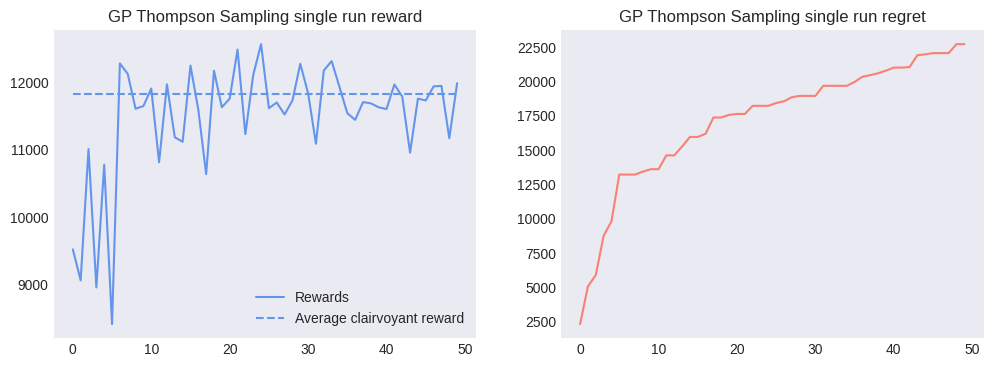
\includegraphics[scale=0.4]{img/Graphs/uncertain_alpha/image1.png}
	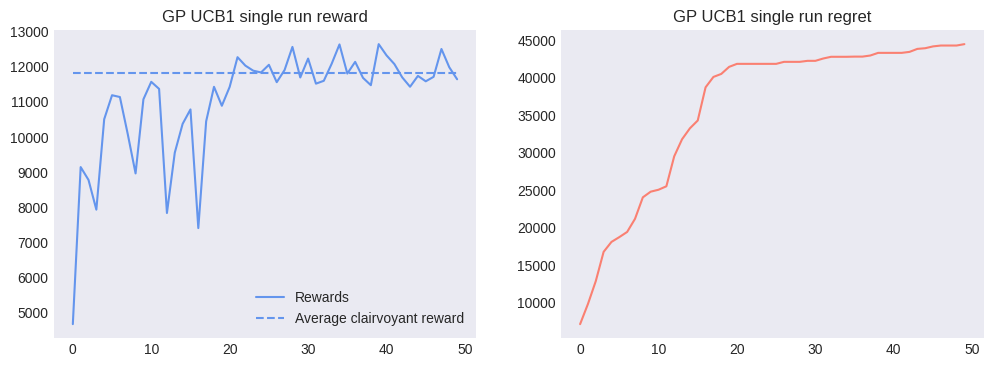
\includegraphics[scale=0.4]{img/Graphs/uncertain_alpha/image2.png}
\end{center}

\end{frame}

% ----------------------------------------

\begin{frame}[plain]

\frametitle{Regret comparison}
\framesubtitle{Thompson Sampling and UCB}

\begin{center}
	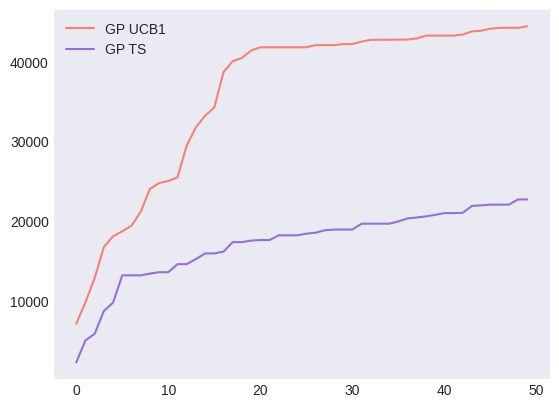
\includegraphics[scale=0.5]{img/Graphs/uncertain_alpha/image3.png}
\end{center}

\scriptsize All tests are done using the \texttt{example\_environment} default values, \textit{population mean} of 1000, \textit{variance} of 10 and 20 \textit{budget steps}.

\end{frame}

% ----------------------------------------

\begin{frame}[plain]

\frametitle{Average regret and reward}
\framesubtitle{Thompson Sampling and UCB}

\begin{center}
	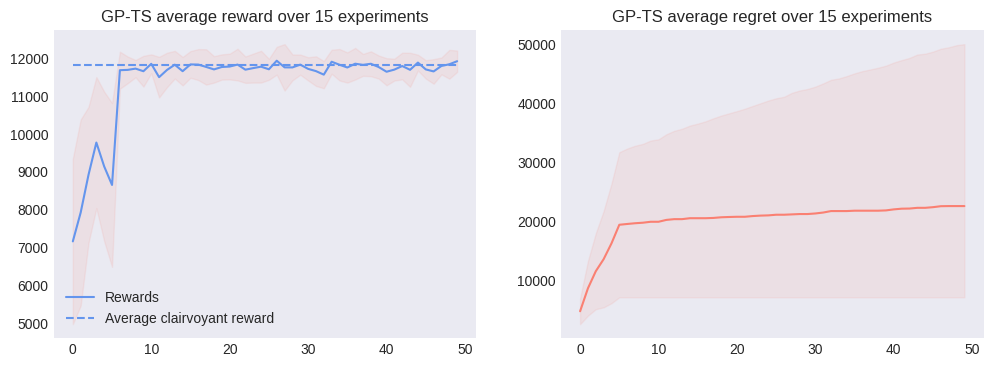
\includegraphics[scale=0.4]{img/Graphs/uncertain_alpha/image4.png}
	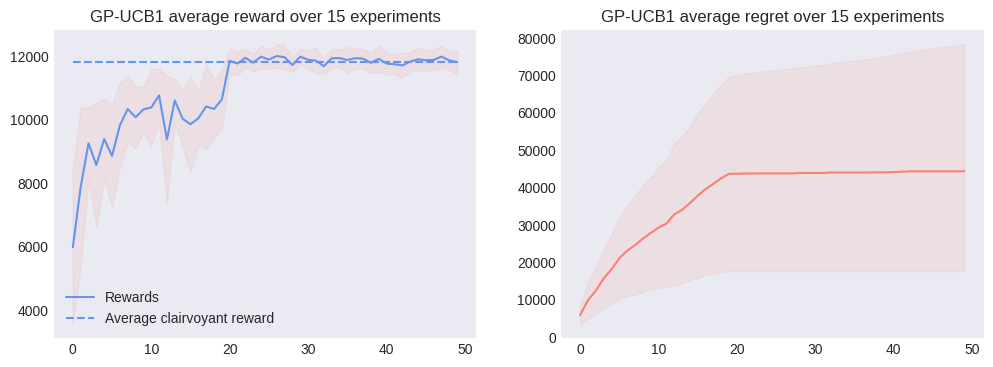
\includegraphics[scale=0.4]{img/Graphs/uncertain_alpha/image5.png}
\end{center}

\end{frame}

% ----------------------------------------

\begin{frame}[plain]

\frametitle{Average regret comparison}
\framesubtitle{Thompson Sampling and UCB}

\begin{center}
	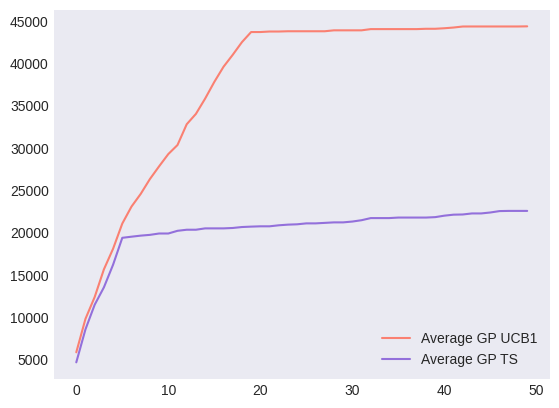
\includegraphics[scale=0.45]{img/Graphs/uncertain_alpha/image6.png}
\end{center}

\begin{displaymath}
	\text{Regret ratio } = \frac{\text{Avg regret}}{\text{Upper bound}} = \frac{31019.4}{?} = ?
\end{displaymath}

\scriptsize Values reference GPTS regret compared to advertising GP regret found at [SLIDE REFERENCE]

\todo{complete}

\end{frame}

% ----------------------------------------

\begin{frame}

\frametitle{Results}

Overall we can observe more instability in the \textbf{TS} algorithm, but a faster convergence w.r.t to the \textbf{UCB} approach.

Both algorithms clearly converge to the optimal solution at different rates while respecting a linear cumulative regret bound.

Average results over 15 runs at time horizon $T = 50$:

\begin{table}
	\begin{tabular}{|c|cc|c|}
	\hline \hline
		\cellcolor{blue!25} & Reward 	& Regret	& Deviation \\
	\cline{2-4}
		\cellcolor{blue!25} & $\mu$		& $\mu$		& $\sigma$	\\
	\hline \hline
		GPTS 				& 11610.53 	& 31024.67	& 440.36 	\\
	\hline
		GPUCB				& 11737.73	& 43686.67	& 349.47	\\
	\hline \hline
	\end{tabular}
\end{table}

\end{frame}

% ----------------------------------------
